% \subsection{Rotationsmatrizen}
%
% \begin{tabular}{ l | l }
% I & II \\ \hline
% IV & III \\
% \end{tabular}
%
% \flushleft
% \hfill
% \begin{tabular}{l | l l}
%   Clockwise & & \\ \hline
%   I & + & + \\
%   II & + & - \\
%   III & - & - \\
%   IV & - & +
% \end{tabular}
% \hfill
% \begin{tabular}{l | l l}
% Anticlockwise & & \\ \hline
% I & - & - \\
% II & - & + \\
% III & + & + \\
% IV & + & -
% \end{tabular}
% \hfill
%
% \subsection{Die Matrizen}
%
% \subsubsection{Rotation um die x-Achse}
%
% \begin{equation}
%   R_x (\alpha) =
%    \begin{pmatrix}
%       1 & 0 & 0 \\
%       0 & cos(\alpha) & -sin(\alpha) \\
%       0 & sin(\alpha) & cos(\alpha)
%     \end{pmatrix}
% \end{equation}
%
% \subsubsection{Rotation um die y-Achse}
%
% \begin{equation}
%   R_y (\alpha) =
%    \begin{pmatrix}
%       cos(\alpha) & 0 & sin(\alpha) \\
%       0 & 1 & 0 \\
%       -sin(\alpha) & 0 & cos(\alpha)
%     \end{pmatrix}
% \end{equation}
%
% \subsubsection{Rotation um die z-Achse}
%
% \begin{equation}
%   R_z (\alpha) =
%    \begin{pmatrix}
%       cos(\alpha) & -sin(\alpha) & 0 \\
%       sin(\alpha) & cos(\alpha) & 0 \\
%       0 & 0 & 1
%     \end{pmatrix}
% \end{equation}

\subsection{Spiralgalaxies}

\subsection{Using Object Oriented Programming (OOP) techniques}

In my case, the objects are galaxies.

\subsubsection{Initialisation}

The galaxy is initialised with the following objects:

\begin{itemize}
  \item A list storing the coordinates of each star
  \begin{itemize}
    \item X Coordinate
    \item Y Coordinate
    \item Z Coordinate
  \end{itemize}

  \item A list storing the individual forces acting on the stars
  \begin{itemize}
    \item X Force
    \item Y Force
    \item Z Force
  \end{itemize}

  \item A variable storing the number of stars generated in the galaxy

  \item Newtons gravitational constant
\end{itemize}

\subsection{Generation of new stars}

The function is given an integer defining the amount of stars that should be
newly generated.

The newly generated stars are then appended to the list storing the coordinates.

The counter counting the amount of stars in the galaxy is incremented.

\subsection{Printing all the coordinates}

The function cycles through the list storing the star coordinates and prints
them to the command line.

\subsection{Calculating the Forces acting between the Stars}

The function recieves two star objects and an axis on which the forces should
be calculated and returns the force acting on the given axis. In case of a
failture (The two given stars have got the same coordiantes), the function
just goes on to the next Star.

The Forces can be calculated using the equation (\ref{eq:gravitation_law}).

\subsection{Calculating the forces acting between each star in the galaxy and
each other star}

To calculate the forces inbetween every star in the galaxy, the function cycles
through every star, looks if the force that should be calculated hat not been
calculated yet and calculates it. This includes testing if the force that should
be calculated is not the force inbetween a star and itself.

The results of the calculations are stored in a list storinf the forces.

\subsection{Printing all the individual forces}

The function is able to print all the forces acting inbetween the stars if no
argument is given. If an argument n is given, the function print out the nth
star in the list.

\subsection{Spherical cells}


\subsubsection{Testing if a point is inside or outside a sphere}

In order to test is a point is inside a sphere, one just has to test if the
following conditions are all true:

\begin{equation}
  \begin{split}
    S_x - S_r \leq P_x \leq S_x + S_r \\
    S_y - S_r \leq P_y \leq S_y + S_r \\
    S_z - S_r \leq P_z \leq S_z + S_r
  \end{split}
\end{equation}

\( P_x \) , \( P_y \) and \( P_z \) are the coordinates of the point to be tested,
\( S_x \) , \( S_y \) and \( S_z \) are the coordinates of the midpoint of the sphere and
\( S_r \) is the radius of the sphere.

\subsubsection{Testing if a star is inside or outside of a sphere for a whole galaxy}

While testting if a star is inside a sphere or not, because of the alignment
of the spheres, a point can be in more than one sphere at the same time.
To get rid of this problem, the software cycles over every star and searches
for matches within the spheres. If a match is found, the next star is tested.
This is pretty much as efficient as it can get.

\begin{equation}
  O(n) = n_{stars} \cdot n_{spheres}
\end{equation}

\subsubsection{Generate the position of the spheres}

Generating the position of the spheres is accomplished in the following way:
A 3D-grid is generated and the midpoints of the spheres are positioned on the
gridpoints.

[Include Graphic]

The distance the spheres have to each other ist defined using the following
function:

\begin{equation} \label{sphere_distance}
  \texttt{sphere\_distance} = \frac{\texttt{galaxy\_range}}{\texttt{sampling\_rate}}
\end{equation}

The higher the \texttt{sampling\_rate} is, the more spheres get generated.

The next goal is to find out the ``sweet spot'' generating the spheres.
When using a very low \texttt{sampling\_rate}, the reault gets inacurate, but
when using a high \texttt{sampling\_rate}, the calculations are not affected
in term of speed and efficiency. The Goal is therefor to find a sampling rate
that enables the generation of accurate but fast results.

By being able to controll the accuracy anf therefor the time, it is possible to
teach the system to generate a galaxy in like one hour and it will automatically
set the sampling rate so low that the simulation will finish perfectly in time.

\subsubsection{The radius of the spheres}

The Radius of the spheres is dynamicly allocated to ensure that the whole galaxy
is covered.

\begin{equation} \label{sphere_radius}
  r = \sqrt{\texttt{sphere\_distance}^2 + \texttt{sphere\_distance}^2 + \texttt{sphere\_distance}^2}
\end{equation}

\begin{equation*}
  1.7320508075688772 = \sqrt{1^2 + 1^2 + 1^2}
\end{equation*}

The equation (\ref{sphere_radius}) highly depends on the equation
(\ref{sphere_distance}) and it's parameters.

\begin{figure}
  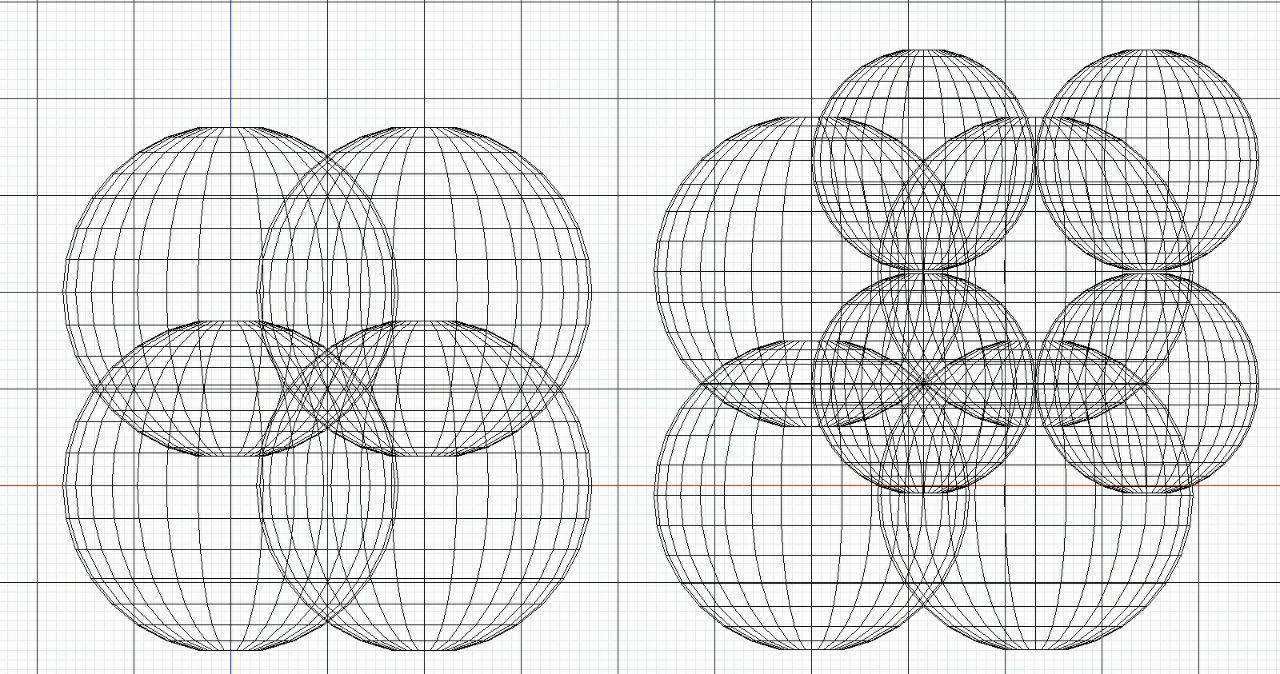
\includegraphics[width=1\textwidth]{figs/sphere_alignment_cc}
  \caption{The Alignment of the spheres\\
  Left: The perfect alignment covering the complete space\\
  Right: A previously generated alignment using small spheres to cover the missing space
  }
  \label{sphere_alignment}
\end{figure}

\subsubsection{Calculate the forces acting on the spheres}

In order to reduce the time that is needed to calculate the forces inbetween
the stars, the stars are subdivided in different cells, in this case spheres.
After all the forces acing inside one sphere are calculated, the forces are
combined and applied to the midpoint of the sphere genrating a new coordinate:
the mean force. The mean force inbetween all the cells can be calculated.

[Include description binary tree]

[Include graphic binary tree]

\subsubsection{Calculate the forces acting on all the spheres together}

This should be 0.

\subsubsection{Benchmarks}

\begin{tabular}{l | l | l | l}
  Nr of Stars & Sample rate & Galaxy Range & Time (s) \\\hline


  100         & 1           & 100          & 0.0814 \\
  75          & 1           & 100          & 0.0499 \\
  50          & 1           & 100          & 0.0295 \\
  25          & 1           & 100          & 0.0116 \\ \hline

  100         & 1           & 100          & 0.0828 \\
  100         & 2           & 100          & 0.0909 \\
  100         & 4           & 100          & 0.1832 \\
  100         & 8           & 100          & 1.1114 \\
  100         & 16          & 100          & 7.6944 \\
  100         & 32          & 100          & 56.5731 \\
  100         & 64          & 100          & 217.7768 \\ \hline

  100         & 1           & 1            & 0.0809 \\
  100         & 1           & 2            & 0.0844 \\
  100         & 1           & 4            & 0.0782 \\
  100         & 1           & 8            & 0.0758 \\
  100         & 1           & 16           & 0.0847 \\
  100         & 1           & 32           & 0.0815 \\
  100         & 1           & 64           & 0.0770 \\

\end{tabular}

The sample rate is the factor that influences the time the most. Knowing this,
it (the sample rate) can be used to controll the time in which a galaxy can
be created.
This is usefull in particular when using some very powerfull mashine with
limited time.

\subsection{Calculate the Position of a Star after a timestep}

Not to be considered:
\begin{itemize}
  \item drag
  \item any kind of resistance
  \item acceleration
\end{itemize}

\subsection{Notes}

\begin{itemize}
  \item Don't search for spheres very far away!
\end{itemize}

\begin{equation}
  % \sum_{lower}^{upper} + \sum_{lower}^{upper} - \sum_{lower}^{upper}
  \sum A_{fi} + \sum B_{fi} - \sum AB_{fij}
\end{equation}

\begin{itemize}
  \item USE dictionaries to store which stars are in wich spheres
\end{itemize}

\subsection{exec.py}

The exec.py file is used to execute the galaxytools defined in galaxytools.py.

\subsubsection{Importing the galaxytools}

\begin{lstlisting}
  import galaxytools as galaxytools
\end{lstlisting}

The complete prgramm is compressed into one object. This Object has to be
imported in order to be used.

\subsubsection{Generate a new galaxy}

\begin{lstlisting}
  galaxy = galaxytools.new_galaxy(100)
\end{lstlisting}

Using the previously imported library, one can start building a galaxy by
calling the function new\_galaxy(...). The parameter inside the braces defines
the size of the galaxy.

\subsubsection{Generate new stars in the galaxy}

\begin{lstlisting}
  galaxy.gen_new_stars(100)
\end{lstlisting}

The function new\_stars(...) is used to generate in given amount of new stars.

\subsubsection{Print the coordinates of every star in the galaxy relative to
the origin}

\begin{lstlisting}
  galaxy.print_stars()
\end{lstlisting}

Printing the coordinates of every star in the galaxy is useful for debugging:
It is clearly visible if something is going wrong on the first look. The
range of the galaxy might be wrong or the whole galaxy might be completely
wrong scaled.

\subsubsection{Calculate the forces acting inbetween all the stars in the
galaxy}

\begin{lstlisting}
  galaxy.calc_all_forces()
\end{lstlisting}

the function calc\_all\_forces() if used to calculate all the forces acting
in the selected galaxy. The O notation for this can be calculated using the
following equation: \( O(n) = n^2 \).

\subsubsection{Print the individual forces acting on the stars}

\begin{lstlisting}
  galaxy.print_individual_forces()
\end{lstlisting}

The individual forces (x, y, z) acting on the star can be printed out too!
Just use the function print\_individual\_forces() and you will recieve the
individual forces nicley formatted.

\subsubsection{Generate the coordinates of the positions for the spheres}

\begin{lstlisting}
  galaxy.gen_sphere_positions(2)
\end{lstlisting}

To generate the sphere positions subdividing the galaxy, the
gen\_sphere\_positions(...) function is utilized. The Parameter defines how
many spheres are generated on one axis of the galaxy, so a higher value equals
more spheres and so a longer time to compute. An infinite high value can be used
if the value between each star should be calculated (use at own risk!).

\subsubsection{Calculate the forces after 1 time step}

\begin{lstlisting}
  galaxy.gen_forces_after_t(1)
\end{lstlisting}

Calculating the new position after one timestep makes it possible to animate
the galaxy and so visualizing it in an exciting way making people think you've
done something awesome! This can be acchieved by using the
gen\_forces\_after\_t(...) function. It uses a timestep as an argument and
uses it to calculate the new coordinates of the star.

\subsection{galaxytools.py}

Inside this file, pretty much everything for building a galaxy is defined.

\subsubsection{Importing important libraries}

\begin{lstlisting}
# Import libraries
import math as math  # general math
import numpy as np  # advanced math
# import matplotlib.pyplot as plt  # plotting things
\end{lstlisting}

This part of the code is used to import libraries which are then used to do
e.g. advanced math.

\subsubsection{Generating the new\_galaxy class}

\begin{lstlisting}
# class used to create galaxies
class new_galaxy(object):
\end{lstlisting}

The class definition defines the galaxytools classname as new\_galaxy

\subsubsection{Initialisation}

\begin{lstlisting}

    # Initialisation
    def __init__(self, galaxy_range):
        print(
            """>>> Initialising the list storing coordinates, forces and other
            values"""
        )

        # list used for storing the coordinates os the stars
        self.list_coords = []

        # list storing the overall force acting on one star
        self.list_force_star = []

        # list storing the coordinates of the midpoints of the spheres dividing
        # the galaxy into equaly big sized cells
        self.list_sphere_coords = []

        # self.list_sphere_stars = np.array(3, )

        print("\tDone\n")
        print(">>> Initialising variables and constants")

        # variable storing the number of stars generated
        self.num_of_stars = 0

        self.galaxy_range = int(galaxy_range)

        # define the universal gravitational constant
        self.G = 6.67408 * 10e11

        print("\tDone\n")

\end{lstlisting}

\subsubsection{Generating new stars}

\begin{lstlisting}

    # generate n new stars and store the coordinates in list_coords
    # n = number of stars to be generated
    # galaxy_range = size of the galaxy
    def gen_new_stars(self, n):
        print(">>> Generating Stars...")

        # for a given number of stars
        for i in range(0, n):

            # generate a temporary random coordinate inside a given range using
            # numpy
            self.temp_coord = np.random.uniform(
                low=0, high=self.galaxy_range, size=(4, ))

            # append the random coordinate to the list storing the coordinates
            self.list_coords.append(self.temp_coord)

        # increment the generated star counter
        self.num_of_stars += n
        print("\tDone")
        print("\tGenerated " + str(n) + " Stars\n")

\end{lstlisting}

\subsubsection{Print out all the star coordinates}

\begin{lstlisting}

    # print out all the coordinates in list_coords
    def print_stars(self):
        print(">>> Listing the coordinates of all stars:")
        # print the coordinates of every star
        for value in self.list_coords:
            print(value)

        print("\tDone\n")

\end{lstlisting}

\subsubsection{Calculate the forces acting inbetween two stars}

\begin{lstlisting}

    # calculate the forces acting between two stars on a specified axis
    # star1 = coordinates of the first star
    # star2 = coordinates of the second star
    # axes = "x", "y" or "z" (CASE SENSITIVE!)
    def calc_forces(self, star1, star2, axes):
        if axes == "x":
            mass = star1[3] * star2[3]
            distance = math.sqrt(math.pow(star1[0] - star2[0], 2))
        elif axes == "y":
            mass = star1[3] * star2[3]
            distance = math.sqrt(math.pow(star1[1] - star2[1], 2))
        elif axes == "z":
            mass = star1[3] * star2[3]
            distance = math.sqrt(math.pow(star1[2] - star2[2], 2))

        # stop division by zero
        if distance == 0:
            pass
        else:
            # return the acting force
            return self.G * mass / math.pow(distance, 2)

\end{lstlisting}

\subsubsection{Calculate all the forces acting in the galaxy}

\begin{lstlisting}

    # calculate all the forces acting in the current galaxy
    def calc_all_forces(self):
        print(">>> Calculating all the forces acting inbetween the stars:")

        if (self.num_of_stars <= 5):
            # print some information above the columns
            print(">>> Printing the forces acting inbetween every star")
            print("{:-<60}".format(""))
            print("\t| {:<3}| {:<3}| ".format("a", "b"))
            print("\t+{:-<4}+{:-<4}+{:-<60} ".format("", "", ""))

        else:
            print("\t[W] Too many stars to print out!")
            print("{:-<60}".format(""))

        # for every star
        for i in range(0, self.num_of_stars):

            # initialize
            self.force = 0

            # every other star:
            for j in range(0, self.num_of_stars):

                # don't calculate the force between a star and and itself
                if i != j and i < j:
                    self.arr_force = np.array((0, 0, 0))

                    # calculate the force between the two stars
                    force_x = self.calc_forces(self.list_coords[i],
                                               self.list_coords[j], "x")
                    force_y = self.calc_forces(self.list_coords[i],
                                               self.list_coords[j], "y")
                    force_z = self.calc_forces(self.list_coords[i],
                                               self.list_coords[j], "z")

                    # print("overall force: ", end="")
                    self.arr_force = np.array((force_x, force_y, force_z))

                    if (self.num_of_stars <= 5):
                        print("\t| {:<3}| {:<3}| {:<60}".format(
                            str(i), str(j), str(self.arr_force)))
                    """
                    force_x = 42
                    force_y = 36
                    force_z = 24

                    (0, 0, 0) --> (42, 36, 24)
                    """

            # append the variable to the list storing all the forces
            self.list_force_star.append(self.arr_force)

        print("{:-<60}".format(""))
        print("\tDone\n")

\end{lstlisting}

\subsubsection{Print the individual forces acting on one star}

\begin{lstlisting}

    # print the individual forces acting on a star
    def print_individual_forces(self, n=None, print_confirm=False):
        print(">>> Printing the individual forces acting on every star")

        if self.num_of_stars > 10:
            print("\t[W] Too many stars to print out!")
            print("{:-<60}".format(""))

            for i in range(0, 3):
                print("\t" + str(i) + " " + str(self.list_force_star[i]))

            print("\n\t...\n")

            for i in range(
                    int(len(self.list_force_star) - 3),
                    len(self.list_force_star)):
                print("\t" + str(i) + " " + str(self.list_force_star[i]))
            print("{:-<60}".format(""))

        else:
            print("{:-<60}".format(""))
            if n is None:
                # for value in self.list_force_star:
                for i in range(0, len(self.list_force_star)):
                    print("\t" + str(i) + " " + str(self.list_force_star[i]))
            else:
                print(self.list_force_star[n])

            print("{:-<60}".format(""))
            print("\tDone\n")

\end{lstlisting}

\subsubsection{Find out if a star is inside one sphere}

\begin{lstlisting}

    # star      [x, y, z, mass]
    # sphere    [x, y, z, radius]
    def is_star_in_sphere(self, star, sphere):

        # define the sphere values
        self.sphere_x = sphere[0]
        self.sphere_y = sphere[1]
        self.sphere_z = sphere[2]
        self.sphere_r = sphere[3]

        # define the star coordinates
        self.star_x = star[0]
        self.star_y = star[1]
        self.star_z = star[2]

        # find out the distance between the point and the center of the sphere
        # if the distance is bigger than the radius of the sphere, the point is
        # not inside the sphere. Elsewise, the point is inside the sphere

        x = math.pow(self.sphere_x - self.star_x, 2)
        y = math.pow(self.sphere_y - self.star_y, 2)
        z = math.pow(self.sphere_z - self.star_z, 2)
        r = math.sqrt(x + y + z)

        if r > self.sphere_r:
            return False
        else:
            return True

        # self.sphere_x_neg = self.sphere_x - self.sphere_r
        # self.sphere_x_pos = self.sphere_x + self.sphere_r
        #
        # self.sphere_y_neg = self.sphere_y - self.sphere_r
        # self.sphere_y_pos = self.sphere_y + self.sphere_r
        #
        # self.sphere_z_neg = self.sphere_z - self.sphere_r
        # self.sphere_z_pos = self.sphere_z + self.sphere_r
        #
        # # find out if the star is inside the sphere
        # if self.sphere_x_neg < self.star_x < self.sphere_x_pos:
        #     if self.sphere_y_neg < self.star_y < self.sphere_y_pos:
        #         if self.sphere_z_neg < self.star_z < self.sphere_z_pos:
        #             return True
        #         else:
        #             return False
        #     else:
        #         return False
        # else:
        #     return False

\end{lstlisting}

\subsubsection{Find out which star in in which spheres}

\begin{lstlisting}

    # find out which stars in in which spheres
    def is_star_in_sphere_all(self):

        # print(self.sphrer_rs)

        print(">>> is_star_in_sphere_all")

        # initialize a temporary counter in order to index the spheres
        tmp_counter = 0

        # cycle through all the stars
        for sphere in self.sphere_coords:
            # print("sphere: " + str(sphere))

            tmp_list = []
            for star in self.list_coords:
                # parse the needed values from the sphere list

                # if the star is inside the sphere
                if (self.is_star_in_sphere(star, sphere) is True):
                    # print("\nstar: " + str(star))

                    star_x = []

                    for value in star:
                        # print(value, end=" ")
                        # print("")
                        star_x.append(value)

                    # print("star_x :" + str(star_x))

                    tmp_list.append(star_x)

            # print("")
            # print("tmp_list: " + str(tmp_list))
            # print("END")

            self.sphere_coords[sphere] = tmp_list

        print("")
        # print(self.sphere_coords)

        # cycle through the dictionary storing which star is in which cell
        for value in self.sphere_coords:
            stars_in_sphere = self.sphere_coords[value]

            # calculate the individual forces in the sphere
            self.calc_forces_sphere(stars_in_sphere)

            # for value in stars_in_sphere:
                # print(value)

\end{lstlisting}

\subsubsection{Generate the sphere positions}

\begin{lstlisting}

    # function generating the positions of the sphere cells
    def gen_sphere_positions(self, sampling_rate):

        print(">>> Generating the sphere positions")

        # initialize a dictionary linking the sphere coordinates to the
        # coordiantes of the stars in the sphere
        self.sphere_coords = {}

        # calculate the distance between the midpoints of the spheres
        sphere_distance = int(round(self.galaxy_range / sampling_rate, 0))

        # define the sphere_radius
        tmp_var = math.pow(sphere_distance, 2)
        sphere_radius = math.sqrt(tmp_var + tmp_var + tmp_var)

        # define a sphere counter for "labeling" the spheres
        tmp_counter = 0

        # cycle through all potential points
        for i in range(-self.galaxy_range, self.galaxy_range, sphere_distance):
            for j in range(-self.galaxy_range, self.galaxy_range,
                           sphere_distance):
                for k in range(-self.galaxy_range, self.galaxy_range,
                               sphere_distance):

                    # generate a temporary array combining all values
                    # temp_arr = np.array((i, j, k, sphere_radius, tmp_counter))
                    tmp_arr = (i, j, k, sphere_radius, tmp_counter)

                    # append the array to the list storing the sphere infos
                    # self.list_sphere_coords.append(temp_arr)

                    # print("temp_arr: " + str(temp_arr))
                    self.sphere_coords[tmp_arr[0:4]] = []

                    # increment the sphere counter
                    tmp_counter += 1

        # print(self.sphere_coords)
        print("\tDone\n")

\end{lstlisting}

\subsubsection{Calculate the forces acting inside the sphere}

\begin{lstlisting}

    def calc_forces_sphere(self, stars_in_sphere):
        print("stars_in_sphere: ", end="")
        print(stars_in_sphere)
        # for value in stars_in_sphere:
        #     self.calc_all_forces(stars_in_sphere)
        #     print(value)

\end{lstlisting}

\subsubsection{calculate the forces acting in every sphere}

\begin{lstlisting}

    def calc_forces_sphere_all():
        # for i in range(0, len(num_of_spheres)):
        #     for star in sphere[i]:
        #         for star_2 in len(0, num_of_stars_in_sphere[i])
        #             a = calc_force(star, star[j])

        pass

    def gen_print_forces_after_t(t):
        pass

    # def all_stars_in_sphere(self, star, se)

\end{lstlisting}

\subsection{GAN}
